%\VignetteIndexEntry{Introduction to DriverProbabilities}
\documentclass{article}
\usepackage{float}
\usepackage[natbibapa]{apacite}
\bibliographystyle{apacite}

\RequirePackage[]{/home/cog/bvanderroest/R/R-3.4.3/library/BiocStyle/resources/tex/Bioconductor2}
\usepackage[noae, nogin]{Sweave}
\title{Introduction to \Biocpkg{DriverProbabilities}}
\author{Bastiaan Van der Roest}
\affil{University Medical Center Utrecht, Utrecht, The Netherlands}
\date{\today}

\usepackage{Sweave}
\begin{document} 
\Sconcordance{concordance:Introduction_to_DriverProbabilities.tex:Introduction_to_DriverProbabilities.Rnw:%
1 5 1 2 2 6 1 1 0 8 1 1 5 36 1 1 4 1 1 1 2 4 0 1 2 11 1 1 3 2 0 1 3 1 0 1 3 4 0 1 2 1 %
1 1 3 2 0 1 3 1 0 1 3 4 0 1 2 2 1 1 3 2 0 1 3 1 0 1 3 4 0 1 2 4 1 1 2 1 0 1 5 6 0 1 2 %
5 1 1 3 2 0 1 3 1 0 1 3 1 0 1 1 3 0 1 2 4 1 1 3 2 0 1 3 4 0 1 2 4 1 1 3 2 0 1 3 4 0 1 %
2 6 1 1 10 12 0 1 2 7 1 1 11 13 0 1 2 6 1 1 2 6 0 1 1 5 0 1 1 6 0 1 2 2 1 1 2 1 0 1 2 %
4 0 1 2 3 1 1 7 6 0 1 1 3 0 1 2 4 1 1 9 11 0 1 2 8 1 1 3 2 0 1 1 12 0 1 2 3 1 1 6 8 0 %
1 2 5 1 1 3 2 0 1 2 4 0 1 2 3 1 1 2 4 0 1 2 3 1 1 8 10 0 1 2 1 10 18 1 1 4 3 0 1 1 12 %
0 1 2 4 1 1 2 4 0 1 2 1 4 8 1 1 3 5 0 1 2 1 7 7 1}


\maketitle

\tableofcontents

\newpage{}


\section{Introduction}

\textit{In vitro} culturing stem cells for application in for instance 
regenerative medicine, takes potential risks on genetic diseases. Genetic 
changes, caused by mutation accumulation during culturing, can lead to many
genetic disorders, including cancer. In cancer, these genetic changes are
mostly on positions which benefit the affected cell, by activating oncogenic
genes. A large number of those positions is already found and can be used to 
calculate a risk on getting the so-called driver mutations. 

During \textit{in vitro} culturing the mitosis rate and doubling time of a cell
population can be monitored, along with the number of mutations per time. Not
only physiological changes can be monitored, also the genetic changes.
Mutation accumulation leaves a spectrum of different mutation types behind in 
the genome, giving potential risks on the mutation types. This spectrum can 
differ between cell types and even between cells of the same type.
Mutations occur in the whole genome, however cells have developed methods to 
protect the important parts of the genome against mutation accumulation. Genomic
regions are in general more depleted in mutations than whole genome, so in order
to predict the risk on mutations in cancer, this depletion has to be taken into
account. 

The package \Biocpkg{DriverProbabilities} is developed to use all of the above
data, that is the mitosis rate, doubling time, mutational spectrum and depletion 
tests, to calculate the number of oncogenic driver mutations occuring during 
culturing of stem cells. Background information of the package is described
in the article found on bioRxiv: 
\url{https://www.biorxiv.org/content/biorxiv/early/2018/09/29/430165.full.pdf}

\newpage{}

\section{Load package}

If you are a first time user, read the README on how to install the package 
from Github. After installation load the package:



\begin{Schunk}
\begin{Sinput}
> library(DriverProbabilities)
\end{Sinput}
\end{Schunk}

\section{Data}

To build a probability model for oncogenic driver mutations, data is needed 
about the cell dynamics and genetics. First store all input data into variables
and then process the data to get it in the right format for modelling.

\subsection{Import data into variables}
Start with importing data about the cell dynamics, including cell type, 
doubling time, mitosis rate etc. To read the data as strings, first set
\texttt{options(stringsAsFactors = F)}. Then set the basic parameters:

\begin{Schunk}
\begin{Sinput}
> # Number of cells at day 0
> init_numb_cells <- 1
> # The length of the whole genome
> wg_length <- 2881033286
> # The percentage of the Coding Sequence of the whole genome
> CDS_perc <- 0.015
\end{Sinput}
\end{Schunk}

The information about which sample is which cell type must be included:
\begin{Schunk}
\begin{Sinput}
> # Set the in vitro cell types
> cell_types <- c("iPS", "liver", "SI")
> # Give the file with sample name and cell type information
> ST <- "Sampletypes.txt"
> # Set the in vivo tissue
> invivo_tissue <- "colon"
\end{Sinput}
\end{Schunk}

Now set the parameters of the cell dynamics:

\begin{Schunk}
\begin{Sinput}
> # Doubling time for cell population in hours
> doubling_time <- list('iPS'=23.08, 'liver'=46 ,'SI'=44.38)
> # Mitosis rate for cell population
> mitosis_rate <- list('iPS'=18, 'liver'=26, 'SI'=26)
> # Mutation rate per genome per doubling
> mutation_rate <- 'mutation_rates.txt'
\end{Sinput}
\end{Schunk}

The time to culture the cells must be given in hours. In order to give the time
in whole factors of generation cycle time, the mitosis rate, the least common
multiplier between the cell types can be used:

\begin{Schunk}
\begin{Sinput}
> library(pracma)
> # Time to culture the cells in hours. Give time in whole factors of 
> # generation cycle time
> t_culture <- Lcm(Lcm(mitosis_rate[['iPS']], mitosis_rate[['SI']]), 
+                  mitosis_rate[['liver']])*10
\end{Sinput}
\end{Schunk}

Furthermore, give the data about the cell genetics, that is the mutational
spectra of \textit{in vitro} and \textit{in vivo} grown cells and the results
of the enrichment/depletion tests from the \Biocpkg{MutationalPatterns}
package.

\begin{Schunk}
\begin{Sinput}
> # File containing the mutational spectrum for all the samples together
> mut_spec_file <- 'Mutation_spectrum_tissue.txt'
> # File containing the mutational spectrum for the in vivo samples
> mut_spec_in_vivo_file <- 'Mutation_spectrum_in_vivo_tot.txt'
> # File containing the enrichment or depletion of the CDS in mutations
> CDS_dep_file_invitro <- 'CDS_gene_regions_distr.txt'
> CDS_dep_file_invivo <- 'CDS_gene_regions_distr_invivo.txt'
\end{Sinput}
\end{Schunk}

To see which mutations are ongenic drivers, import a catalog with oncogenic
mutations, along with a file in which for each gene the mode of action is 
given.

\begin{Schunk}
\begin{Sinput}
> # File containing validated oncogenic mutations
> oncogenic_mutations <- 'catalog_of_validated_oncogenic_mutations.tsv'
> # File containing activity of driver genes while mutated
> gene_MoA <- 'gene_MoA.tsv'
\end{Sinput}
\end{Schunk}

As final input, state if you want to calculate the probabilities on oncogenic
driver mutations per gene or over all genes. If per gene is wanted, specific 
genes can be selected:

\begin{Schunk}
\begin{Sinput}
> # Select if you want probabilities per gene of all genes at once
> prob_per_gene = F
> # Give a vector of the genes for which you want to visualize the probabilities
> wanted_genes = 'all'
\end{Sinput}
\end{Schunk}

\subsection{Process data into the modelling format}

To process the data to have it in the right format for using the model, the
function \texttt{processData} can be runned. All needed variables for
downstream functions will be stored in the global environment:

\begin{Schunk}
\begin{Sinput}
> processData(mutation_rate_file = mutation_rate,
+             oncogenic_mutations_file = oncogenic_mutations,
+             gene_MoA_file = gene_MoA,
+             CDS_dep_invitro_file = CDS_dep_file_invitro,
+             CDS_dep_invivo_file = CDS_dep_file_invivo,
+             sample_celltypes_file = ST,
+             invivo_tissue = invivo_tissue,
+             mut_spec_invitro_file = mut_spec_file,
+             mut_spec_invivo_file = mut_spec_in_vivo_file)
\end{Sinput}
\end{Schunk}

Per default, the newly made list \texttt{driver\_counts} will contain counts
of six single nucleotide variants ("C>A", "C>G", "C>T", "T>A", "T>C", "T>G"). 
It is also posible to give counts of the 96 mutation spectrum, taken the 5' and
3' prime nucleotide of a mutation basepair into account. Therefore run the 
\texttt{processData} function with the \texttt{trinucleotide} argument set to 
\texttt{True}:

\begin{Schunk}
\begin{Sinput}
> processData(mutation_rate_file = mutation_rate,
+             oncogenic_mutations_file = oncogenic_mutations,
+             gene_MoA_file = gene_MoA,
+             trinucleotide = T,
+             CDS_dep_invitro_file = CDS_dep_file_invitro,
+             CDS_dep_invivo_file = CDS_dep_file_invivo,
+             sample_celltypes_file = ST,
+             invivo_tissue = invivo_tissue,
+             mut_spec_invitro_file = mut_spec_file,
+             mut_spec_invivo_file = mut_spec_in_vivo_file)
\end{Sinput}
\end{Schunk}

This manual will continue with the six mutation types. 

A check must be done to see if the cell types in the given files were spelled 
in the same way. If this is not the case, the model can take the wrong data
for the cell types. 

\begin{Schunk}
\begin{Sinput}
> cell_types
\end{Sinput}
\begin{Soutput}
[1] "iPS"   "liver" "SI"   
\end{Soutput}
\begin{Sinput}
> names(probs_snv)
\end{Sinput}
\begin{Soutput}
[1] "IPS"     "SI"      "liver"   "In_vivo"
\end{Soutput}
\begin{Sinput}
> names(CDS_dep)
\end{Sinput}
\begin{Soutput}
[1] "Liver"           "iPS"             "Small_Intestine"
\end{Soutput}
\end{Schunk}

Change the names if necessary:

\begin{Schunk}
\begin{Sinput}
> names(probs_snv)[names(probs_snv)=="IPS"] <- "iPS"
> names(CDS_dep)[names(CDS_dep) %in% c("Liver","Small_Intestine")] <- c("liver",
+                                                                       "SI")
\end{Sinput}
\end{Schunk}

The list \texttt{driver\_counts} can be extended with genes which are not in 
the given catalog:

\begin{Schunk}
\begin{Sinput}
> driver_counts[['TP53']] <- table(c("C>T","C>T",
+                                    "C>T","C>G",
+                                    "C>T","C>T",
+                                    "T>C","C>T",
+                                    "C>A","C>T",
+                                    "C>A"))
> driver_counts[['BRAF.V600E']] <- table("T>A")
\end{Sinput}
\end{Schunk}

If only driver counts of genes not present in the catalog must be analyzed, 
it is optional to not fill the \texttt{driver\_counts} list with 
\texttt{processData}: 

\begin{Schunk}
\begin{Sinput}
> processData(mutation_rate_file = mutation_rate,
+             process_drivers = F,
+             CDS_dep_invitro_file = CDS_dep_file_invitro,
+             CDS_dep_invivo_file = CDS_dep_file_invivo,
+             sample_celltypes_file = ST,
+             invivo_tissue = invivo_tissue,
+             mut_spec_invitro_file = mut_spec_file,
+             mut_spec_invivo_file = mut_spec_in_vivo_file)
\end{Sinput}
\end{Schunk}

\section{\textit{In vitro} mutation accumulation}
\subsection{Calculate the results}

Once all the prerequired data is loaded and processed, the results for the 
\textit{in vitro} mutation accumulation can
be calculated with the \texttt{probDriverMut} function. Here, you can give the
cell types and genes for which the results must be calculated. 

\begin{Schunk}
\begin{Sinput}
> invitro_res <- probDriverMut(cell_types = cell_types, 
+                              genes = names(driver_counts))
> head(invitro_res)
\end{Sinput}
\begin{Soutput}
      cells         muts        probs cell_type gene stat
1  1.000000 0.000000e+00 0.000000e+00       iPS  all mean
2  1.717007 1.057971e-07 6.347887e-07       iPS  all mean
3  2.948113 2.874514e-07 1.089936e-06       iPS  all mean
4  5.061932 5.993532e-07 1.871428e-06       iPS  all mean
5  8.691373 1.134891e-06 3.213253e-06       iPS  all mean
6 14.923149 2.054413e-06 5.517172e-06       iPS  all mean
\end{Soutput}
\end{Schunk}

The statistics type (mean, mean minus standard deviation or mean plus standard
deviations) can be also be given as a vector.

\begin{Schunk}
\begin{Sinput}
> invitro_res <- probDriverMut(cell_types = cell_types, 
+                              genes = names(driver_counts), 
+                              stat_type = c("mean",
+                                            "mean-std",
+                                            "mean+std"))
\end{Sinput}
\end{Schunk}

\subsection{Plot the results}

Before the results will be plotted, set the type of mutations and cell types in
the order you want:

\begin{Schunk}
\begin{Sinput}
> invitro_res$cell_type <- factor(invitro_res$cell_type, 
+                                 levels = c("liver", "SI", "iPS"))
> invitro_res$gene <- factor(invitro_res$gene, 
+                            levels = c("all", "TP53", "BRAF.V600E"))
\end{Sinput}
\end{Schunk}

Calculate the intersections of all plotted with a given horizontal line with
the function \texttt{calcIntersects}:

\begin{Schunk}
\begin{Sinput}
> xintersects <- calcIntersects(r = invitro_res, hline = 1)
\end{Sinput}
\end{Schunk}

Then plot the results, along with the horizontal and vertical lines and save
the figure as pdf with the filename given in \texttt{pdf\_out}:

\begin{Schunk}
\begin{Sinput}
> plotMutationsPerCell(invitro_res, 
+                      xmax = 1e13,
+                      ymax = 1e1,
+                      hline = 1,
+                      vline = xintersects,
+                      ylab = 'Number of mutations',
+                      pdf_out = pdf_out)
\end{Sinput}
\end{Schunk}


\begin{figure}[H]
\begin{center}
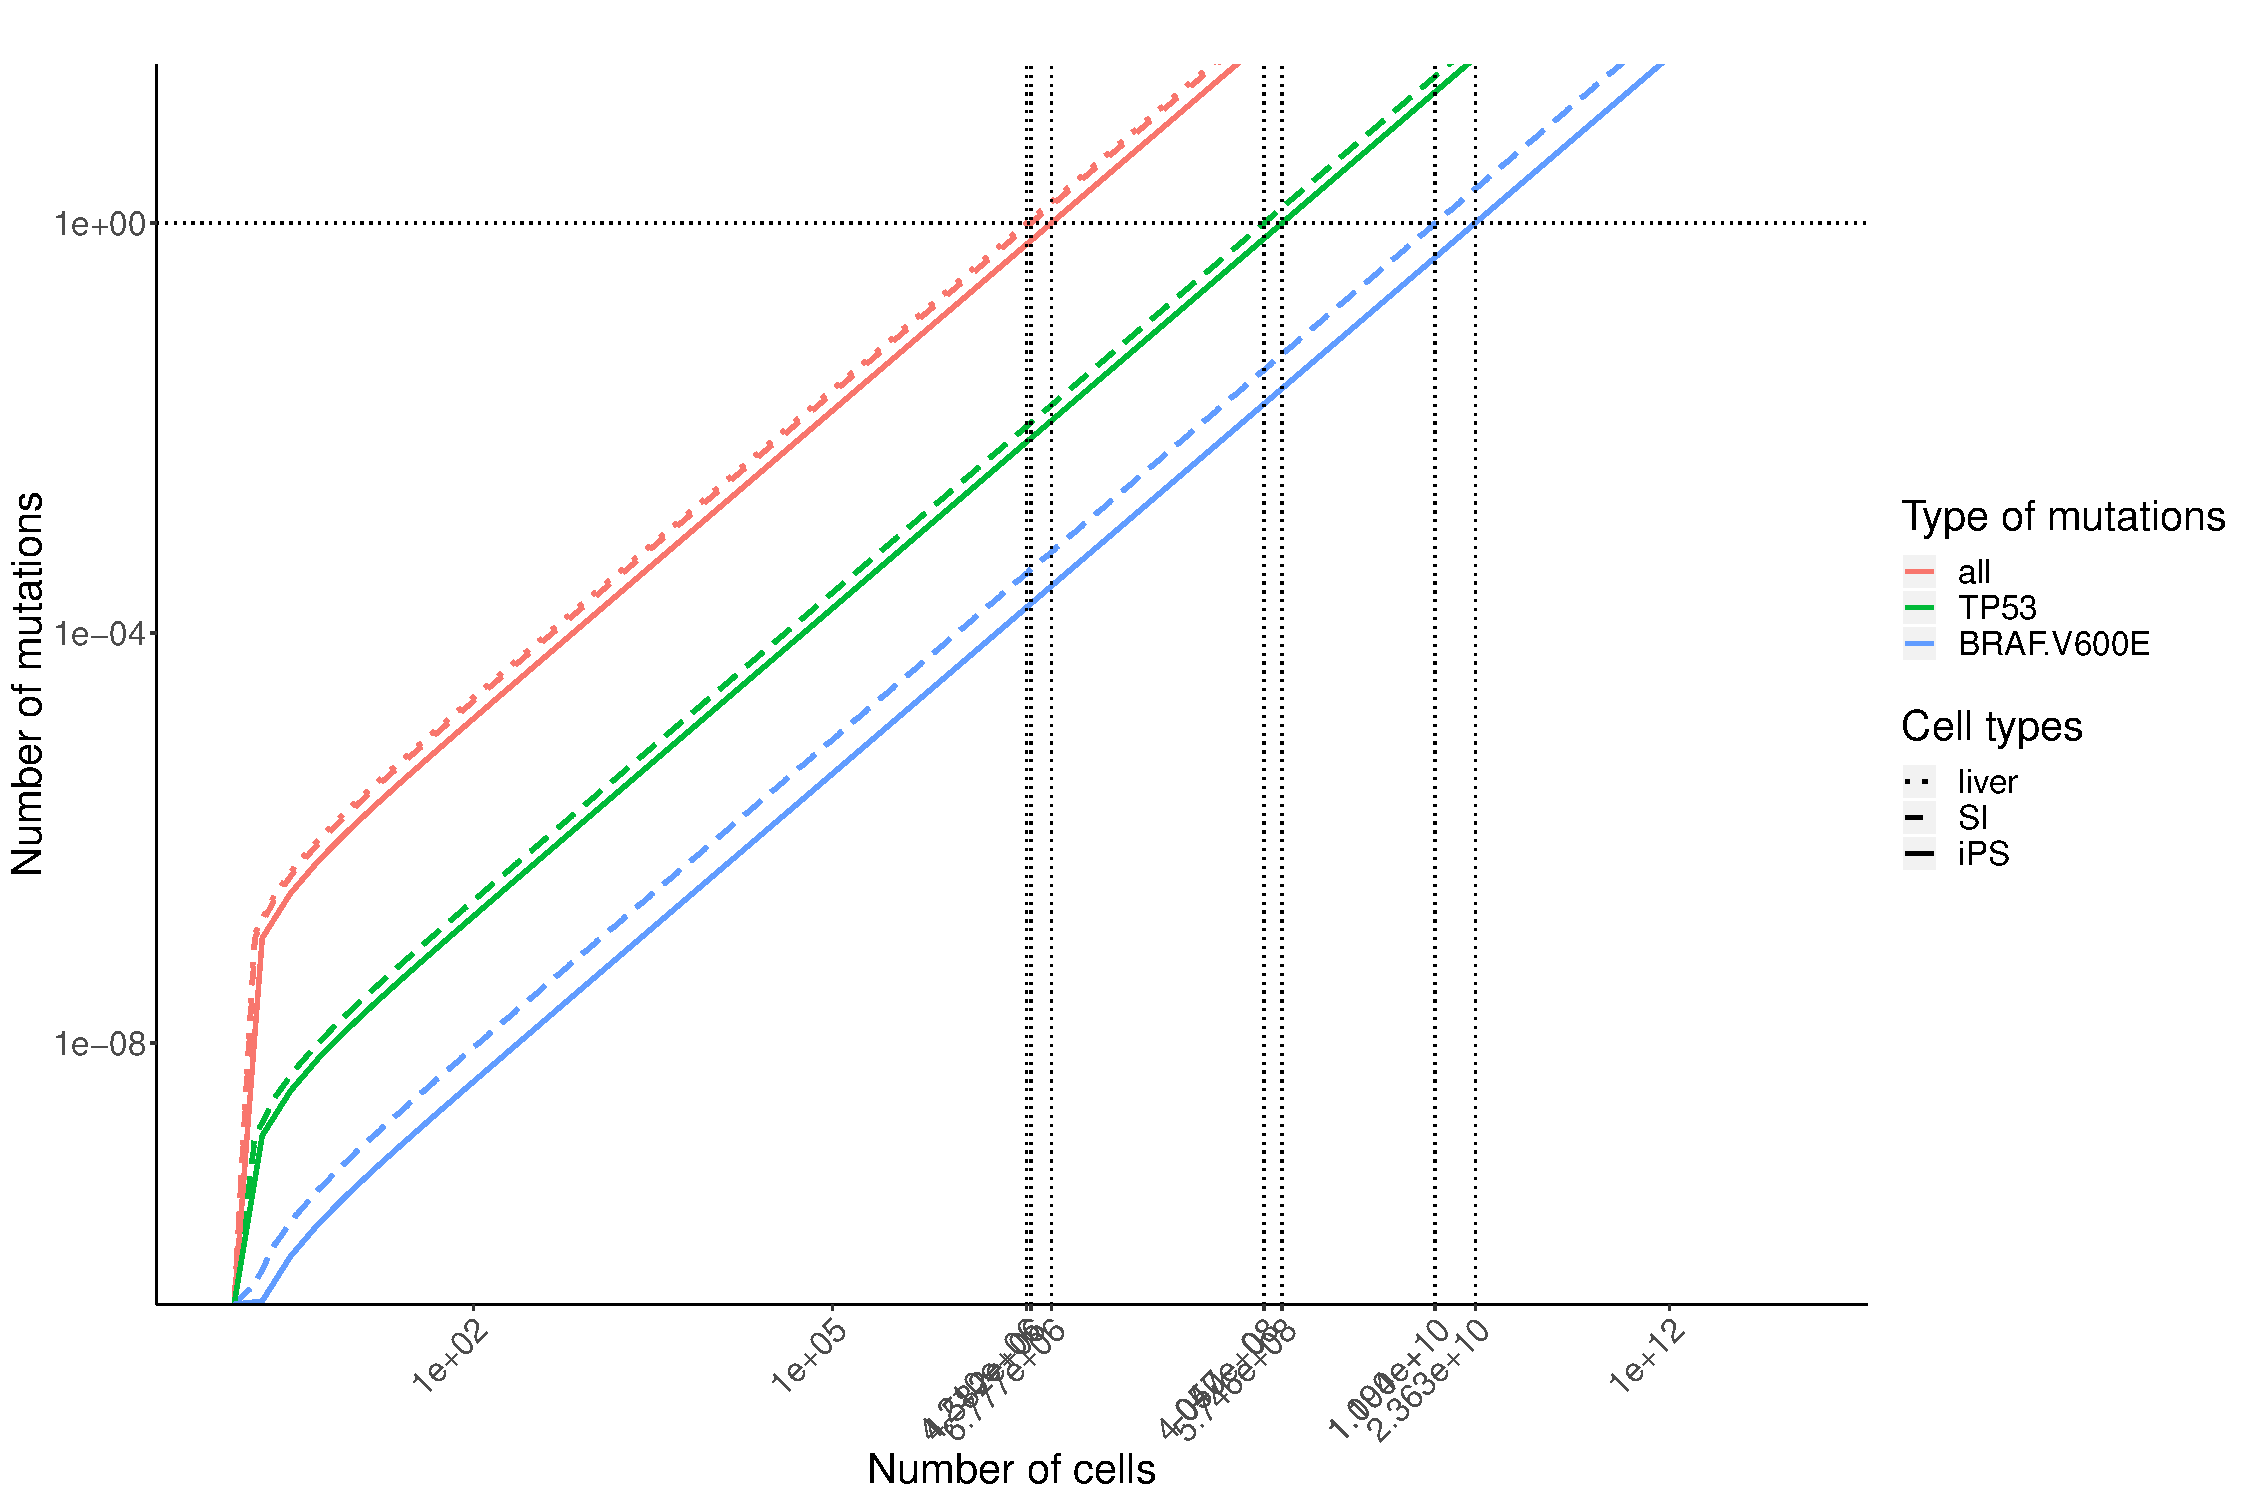
\includegraphics[width=1.0\textwidth]{All_types}
\end{center}
\end{figure}

\newpage{}

\section{\textit{In vivo} mutation accumulation}

To place the results of the \textit{in vitro} mutation accumulation
in context, results from \textit{in vivo} mutation accumulation can be plotted
compared with the mutations from \textit{in vitro} growth, based on the 
probability to gain at least one oncogenic driver mutation. The function 
\texttt{invivoYears} will extend the results from \texttt{probDriverMut} with
the amount of year of \textit{in vivo} mutation accumulation and define two
functions to confer number of cells into years:

\begin{Schunk}
\begin{Sinput}
> invitro_res <- invivoYears(invitro_res, gene = "all", 
+                            dep_invitro = CDS_dep, 
+                            CDS_length = CDS_length[["SI"]])
> head(invitro_res)
\end{Sinput}
\begin{Soutput}
      cells         muts        probs cell_type gene stat         year
1  1.000000 0.000000e+00 0.000000e+00       iPS  all mean 0.000000e+00
2  1.717007 1.057971e-07 6.347887e-07       iPS  all mean 3.144452e-09
3  2.948113 2.874514e-07 1.089936e-06       iPS  all mean 5.399046e-09
4  5.061932 5.993532e-07 1.871428e-06       iPS  all mean 9.270201e-09
5  8.691373 1.134891e-06 3.213253e-06       iPS  all mean 1.591700e-08
6 14.923149 2.054413e-06 5.517172e-06       iPS  all mean 2.732960e-08
\end{Soutput}
\end{Schunk}

Results can be plotted with \texttt{plotInvivoResults} and saved as pdf with 
the filename given in \texttt{pdf\_out}. Per default, \texttt{gene = all} will
be used.

\begin{Schunk}
\begin{Sinput}
> plotInvivoResults(invitro_res, pdf_out = pdf_out)
\end{Sinput}
\end{Schunk}


\begin{figure}[H]
\begin{center}
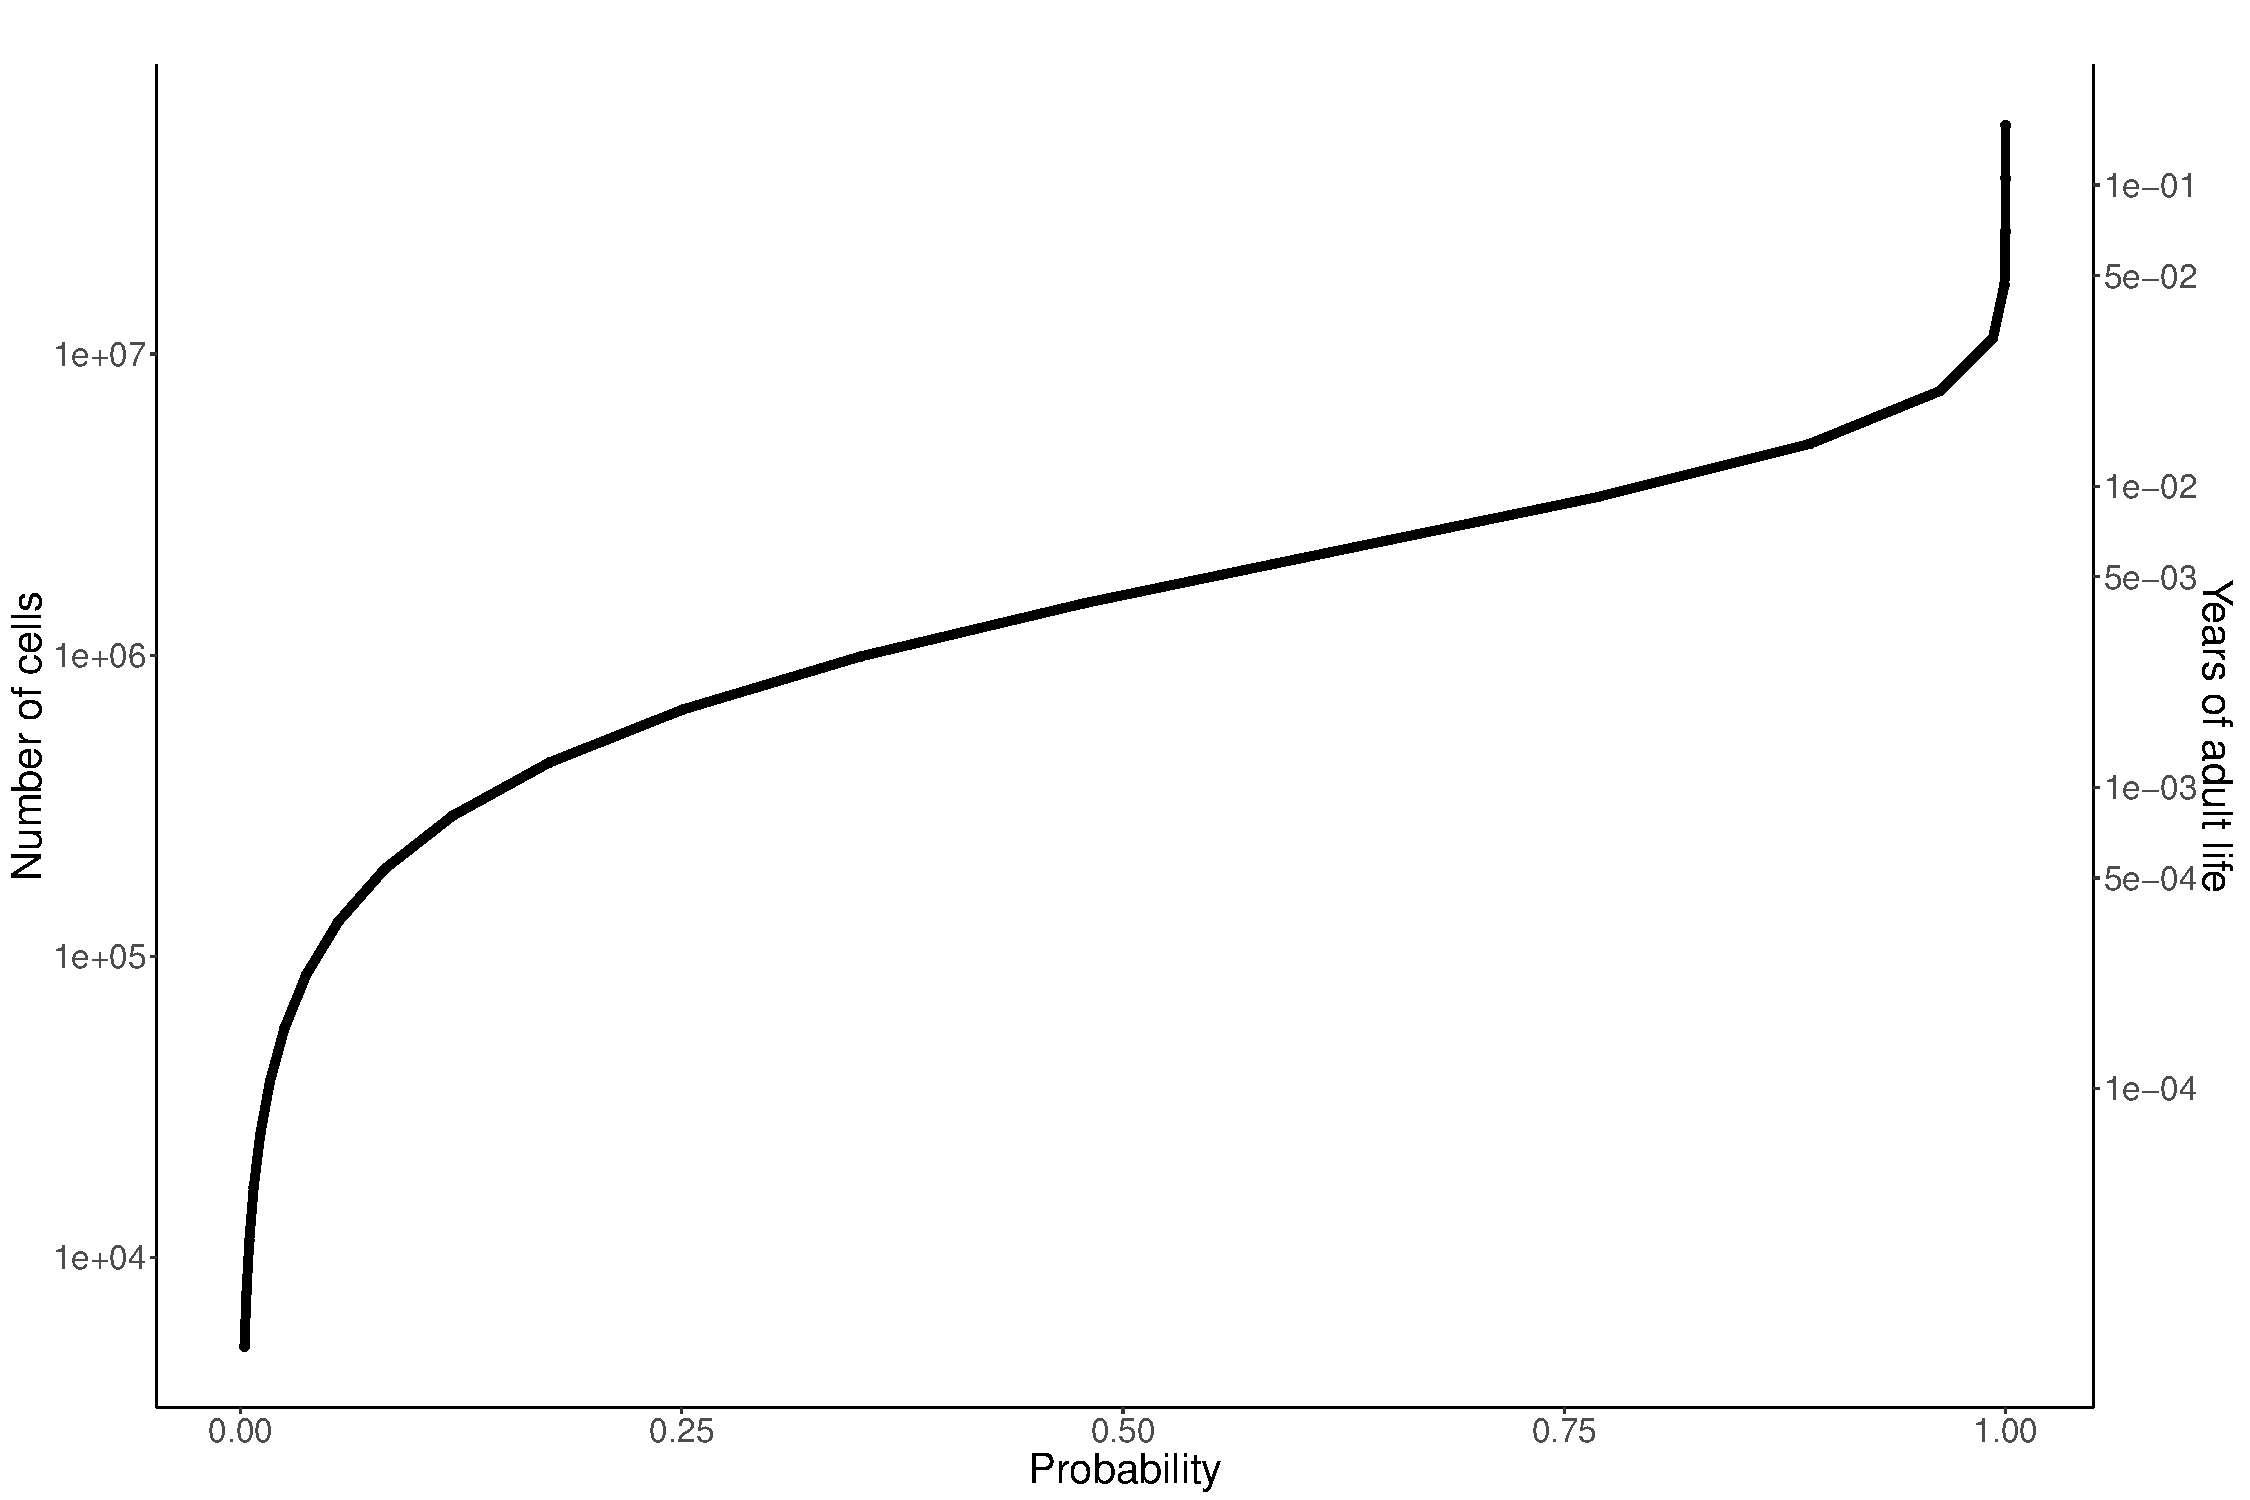
\includegraphics[width=1.0\textwidth]{invivo_all}
\end{center}
\end{figure}

Plot also the results of the "BRAF.V600E" mutation:

\begin{Schunk}
\begin{Sinput}
> plotInvivoResults(invitro_res, gene = "BRAF.V600E", pdf_out = pdf_out,
+                   color = "green")
\end{Sinput}
\end{Schunk}


\begin{figure}[H]
\begin{center}
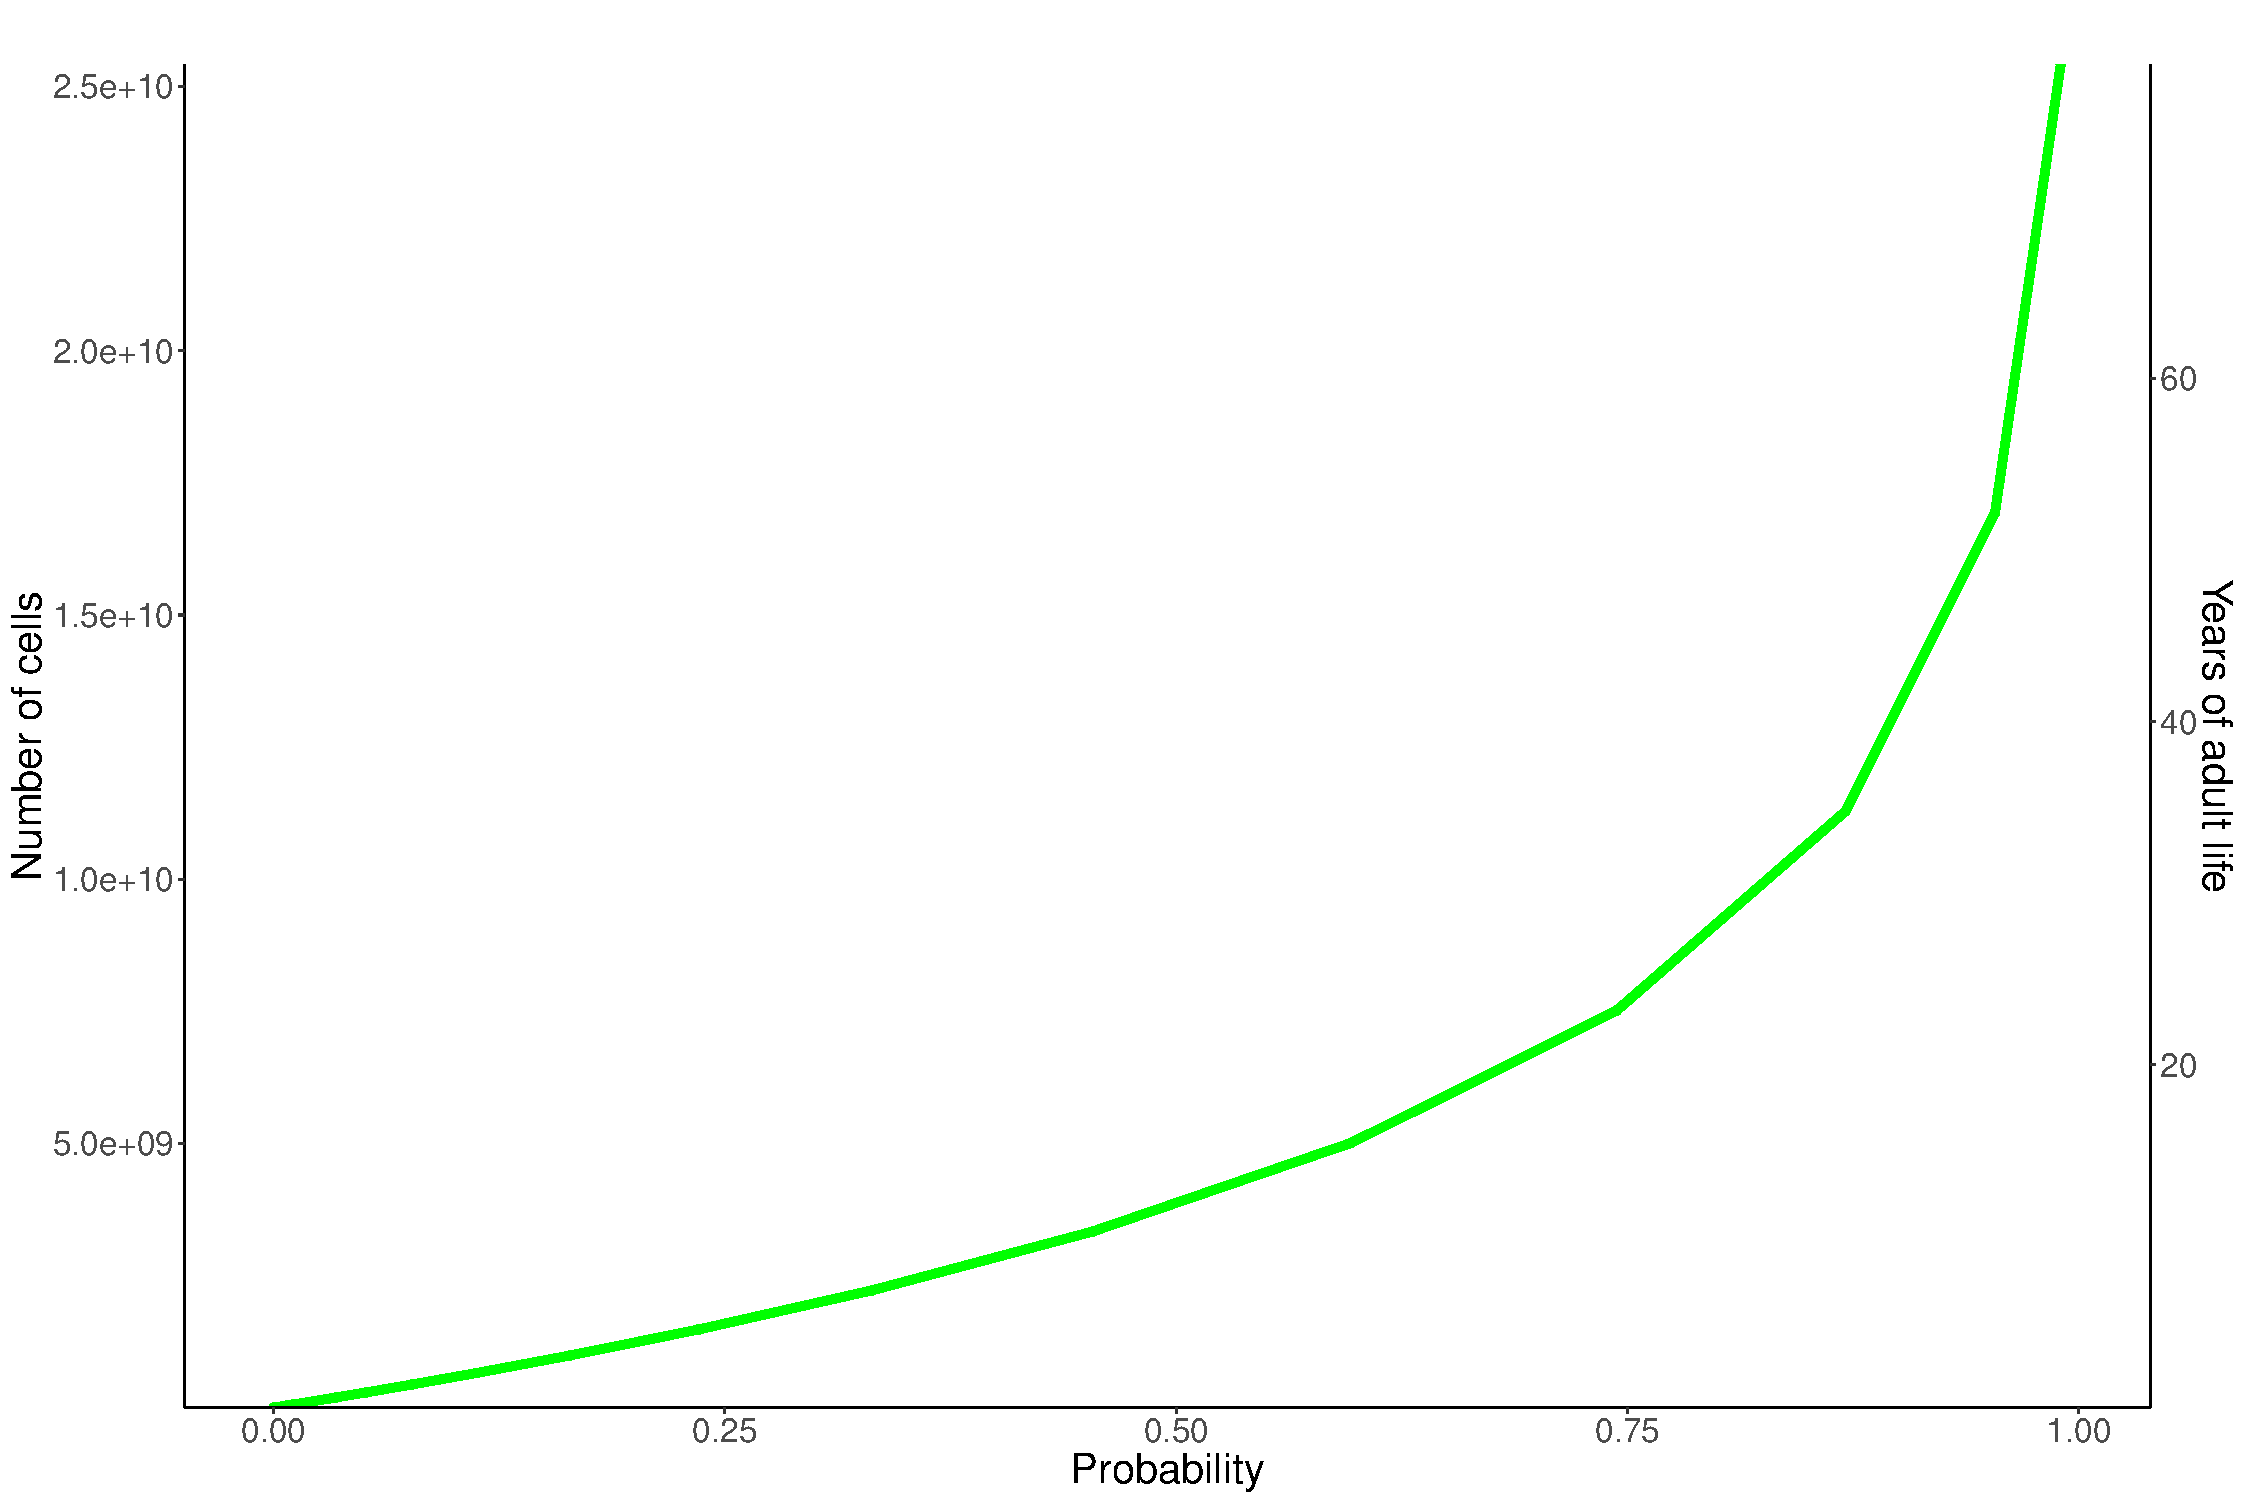
\includegraphics[width=1.0\textwidth]{invivo_BRAF}
\end{center}
\end{figure}

\end{document}
